\subsection{Asymptotic Resilience}

Throughout this subsection, we will assume that $x_\ast$ is a stable rest point of an ODE. Probably the most classical and commonly used mathematical definition of resilience, originally developed by theoretical ecologists\todo{citation}, represents long-term return rates to $x_{\ast}$, and is measured by the dominant eigenvalue at linearization. 

\begin{definition}
	\label{def:asymp}
	 Let $\textbf{A} = Df(x_\ast)$ denote the Jacobian, and recall that all eigenvalues of $\mathbf{A}$ have negative real part. Let $\lambda_1(\textbf{A})$ be the eigenvalue with largest (closest to 0) real part. 
	
	\begin{center}
	The \textbf{asymptotic resilience} of the system at the stable rest point is $Re(\lambda_1(\textbf{A}))$.
	\end{center}
Note: we will refer to $\lambda_1$ as the \textbf{dominant eigenvalue} of $\mathbf{A}$. 
	 \qed 
\end{definition}

For the linearized system $x'= \textbf{A}x$, asymptotic resilience estimates the rate at which trajectories approach the equilibrium. The following theorem is standard theory for linear ODEs. See for example (Chicone p. 175) \todo{do citation}

\begin{theorem}
	If all eigenvalues of an $n \times n$ matrix $\mathbf{A}$ have negative real part, and if $Re(\lambda) < L < 0$ for all eigenvalues $\lambda$ of $A$, then there is some constant $C>0$ such that for all $x \in \mathbb{R}^n$ and $t \geq 0$,
	
	$$|e^{tA}x| \leq Ce^{L t}|x|.$$  \qed
\end{theorem}

Note the expression $e^{tA}x$ in the left hand side is exactly the flow for the linear system $x' = \mathbf{A}x$. So this theorem says that trajectories must decay to the origin, where there is an equilibrium, at an exponential rate. Further, a bound on that rate is governed by the asymptotic resilience. If the equilibrium represents a steady state, then a small perturbation to a system at steady state can be conceptualized as a point which is very close to, but not quite at the equilibrium. Hence, the decay rate represents the rate of recovery from perturbation. 

For nonlinear systems, a similar bound on decay rate is justified by the Stable Manifold Theorem, a fundamental result in dynamical systems theory which says that, for sufficiently nice rest points, the linear approximation based at that rest point is a good approximation. %, also a standard theoretical result. 
%
%The theorem states that there is a local  Moreover, the flow restricted to the stable and the unstable manifolds has exponential (hyperbolic) estimates similar to the inequalities in display (4.1)
%
%
A statement of the Stable Manifold Theorem is built up below. 

\begin{definition}
	Let $A: \mathbb{R}^n \to \mathbb{R}^n$ be a linear transformation. Define the \textbf{stable eigenspace} of $\mathbf{A}$ to be the subspace of $\mathbb{R}^n$ spanned by those eigenvectors of $\mathbf{A}$ with negative real part. Similarly, define the \textbf{unstable eigenspace} of $\mathbf{A}$ to be the subspace of $\mathbb{R}^n$ spanned by those eigenvectors of $\mathbf{A}$ with positive real part. %Finally, define the \textbf{center eigenspace} of $\mathbf{A}$ to be the subspace of $\mathbb{R}^n$ spanned by those eigenvectors of $\mathbf{A}$ with real part exactly equal to zero. 
	\qed
\end{definition}

Note in the case that $\mathbf{A}$ has no eigenvalues with real part equal to 0, it can be decomposed into a direct sum of linear subspaces $\mathbf{A} = E_s \oplus E_u$. In this case we call $\mathbf{A}$ \textbf{hyperbolic}.

\begin{definition}
	Let $x' = f(x)$ be an ODE with $f:U \subset \mathbb{R}^n \to \mathbb{R}^n$, local flow $\phi_t$, and a rest point at $x_0$. The \textbf{stable manifold} $M^s$ %and \textbf{unstable manifold} $M^u$ 
	of $x_0$ is %are defined by
	$$M^s = \{x \in U ~|~ \lim\limits_{t \to \infty} \phi_t(x)= x_0\}$$ 
	%$$M^u = \{x \in U ~|~ \lim\limits_{t \to -\infty} \phi_t(x)= x_0\}$$ 
	\qed
\end{definition}

%\begin{definition}
%	If the center eigenspace of $\mathbf{A}$ is empty, then we say $\mathbf{A}$ is hyperbolic. 
%\end{definition}

\begin{theorem}(Stable Manifold Theorem)
	Consider a non-linear system 
	%
	$$x' = \mathbf{A}(x) + h(x),$$ 
	%
	where $\mathbf{A}, h: \mathbb{R}^n \to \mathbb{R}^n$ with $\mathbf{A}$ linear.  Let $\phi_t$ be the local flow.
	%
	Assume $h(0) =  Dh(0)=0$ so that there is a rest point at the origin. Let $M^s$ be the stable manifold of the origin. 
	%
	Also suppose $\mathbf{A}$ has no eigenvalues with real part equal to 0. Let $E_s$ and $E_u$ be the stable and unstable eigenspaces of $\mathbf{A}$, respectively, so that $\textbf{A} = E_s \oplus E_u$. Let $P_s: \mathbb{R}^n \to E_s$ %and $P_u: \mathbb{R}^n \to E_u$ 
	be the linear projection operator onto the stable %and unstable 
	eigenspace. Also let $\lambda_1$ be the dominant eigenvalue of $E_s$. 
	
	Then there exists a ball $B_\delta(0) \subset \mathbb{R}^n$ about the origin, 
	%
	an $\epsilon > 0$, 
	%
	and a function $\alpha: B_\delta \cap E_s \to E_u $ with $\alpha(0)  = D\alpha(0) = 0$ 
	%
	so that its graph $M^s_{loc} = \{(x, \alpha(x)) \in \mathbb{R}^n : x \in B_\delta \cap E_s\}$ is a \textbf{local stable manifold} of the origin. 
	%
	That is, $$M^s_{loc} = \{x \in U : |P^s(x)| \in B_\delta(0)\} \cap M^s$$
	
	Furthermore, for any $Re(\lambda_1) < L < 0$, there exists $C >0$ such that for all $x \in M^s_{loc}$, $t \geq 0$,
	%
	$$|\phi_t(x)| \leq Ce^{Lt}|x|$$ \qed
\end{theorem}

For a stable rest point, we have $\mathbf{A} = E_s$ because all eigenvalues have negative real part; hence the local stable manifold $M^s_{loc}$ is just a small neighborhood of the rest point. So the bound on decay rate stated in the last line of the theorem implies that any trajectory beginning sufficiently close to equilibrium decays toward equilibrium at an exponential rate, and a bound on that rate is governed by the asymptotic resilience.

%Hence, asymptotic resilience bounds the rate of return to equilibrium after a small perturbation to the system. Because local bifurcation is characterized by $Re(\lambda_1)$ passing through zero, the system recovers slower when nearer to bifurcation. This is the core idea of critical slowing down, which will be explained further in Section \ref{sec:csd}.

\begin{remark}
	Note that trajectories need not decay monotonically in distance to the rest point, not even for linear systems. For instance, a trajectory can initially amplify in magnitude -- a phenomenon termed \textbf{reactivity} by Neubert and Caswell in \cite{neubertAlternativesResilienceMeasuring1997a} (Figure \ref{fig:reactivity}). However, with some large enough choice of $C$, the Stable Manifold Theorem still implies some exponentially decaying bound on the rate of return to equilibrium. 
\end{remark}

\begin{figure}[ht]
	\centering
	\captionsetup{width=0.8\linewidth}
	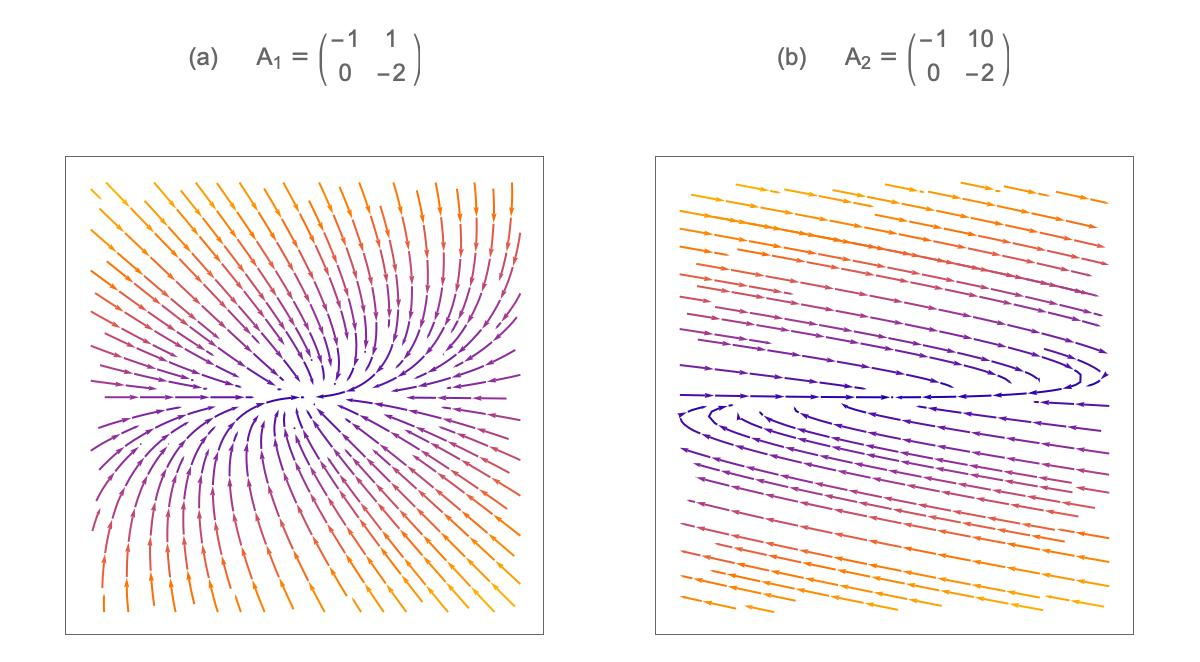
\includegraphics[width=0.8\textwidth]{figs/positive_reactivity_real_example}
	\caption{Phase portraits of two linear systems $x' = \textbf{A}x$ with the same eigenvalues  $\lambda = -1, -2$. (a) All trajectories decay monotonically in magnitude. (b) There are trajectories beginning arbitrarily close to the origin which initially increase in magnitude. Example reproduced from \cite{neubertAlternativesResilienceMeasuring1997a}.}
	
	\label{fig:reactivity}
\end{figure} 